\section{Design}
\label{sec:design}
Stitch~\cite{Bowers_2023stitch} uses a corpus guided top down search approach directly, which works on the lisp-like programs expected by Stitch, but the approach naively fails in \tocheck{imperative languages} due to correctness issues: extracted common subtrees may not, in fact, be valid in the original language.

For example, when Stitch is given a Python's abstract syntax tree (AST) represented in a lisp style, 
% (tweaked to have a lisp-like lambda format) 
some elements or expressions, like the keywords "while" and "if", or operators like "==" and ">", are treated as first-class citizens of the programming language --- extracted subtrees could contain variables that hold such values, or functions could be called with these elements as parameters, resulting in syntactically incorrect calls, 
e.g.\ \texttt{compare(1,2,==)} or assignments, e.g.\ \texttt{x = while}.
% either variable names or function names depending the lamlispifying implementation.
Broadly, this issue arises because Stitch assumes a regular lambda calculus represented in a lisp style, and a Python AST is not sufficiently regular. 
% So, it has no knowledge of what would be a valid abstraction in a language like Python. 

% is unaware of the programming language it is abstracting over, but instead 
% This can result in incorrect abstractions, like an abstraction that expects "if" or "while" as arguments and treats them as variables. Hence, 
% To better generalize Stitch and extend it to a language like Python, we identify and prune such invalid abstractions. 
\toolname{} extends Stitch to correctly extract a library from a corpus of the language \ptwo{}, a large formal subset of Python 3 developed by Siek and Chang~\cite{pythonbook} in their textbook for compiler instruction. All \ptwo{} programs are valid Python 3 programs with equivalent behavior.  The \ptwo{} language supports imperative-style programming, with scoped variable assignment, control, function calls and non-nested definitions.  The language is dynamically typed across integer, booleans, lists, and dictionaries, with support for corresponding operations and comparisons.  Output is done through the \texttt{print} keyword, and input handled via a fixed expression \texttt{eval(input())}, which takes user input, represented as an unsupported string type, and casts it to the appropriate type (e.g.\  if the user inputs \texttt{``True''}, the return value of the corresponding \texttt{eval(input())} expression will be the boolean \texttt{True} value).  The full grammar of the \ptwo{} we support is reproduced in the appendix --- we differ from the full published \ptwo{} only in dropping support for lambdas and nested function definitions, which remain as future work.

The architecture of our \toolname{} tool is shown in Figure ~\ref{fig:design}. As input,
\toolname{} expects in a corpus of \ptwo{} programs.  In the first step (\emph{lispify}), it converts the \ptwo{} programs into a lisp-like format recognizable to Stitch~\cite{Bowers_2023stitch}.  Stitch then proposes a lisp-like candidate for extraction.  The candidate is subsequently subjected to a series of \emph{pruning} checks that verify that the candidate can, indeed, be converted into a valid \ptwo{} function.  These checks correspond with a variety of issues that arise from Python's lack of regularization, and we describe them in depth in the following sections.  Once the candidate is verified, we use liveness analysis to add necessary parameters and return values --- this \emph{closing} is needed to handle the scope of live-in and live-out values from the candidate.  The final step is to \emph{validate call sites} to ensure no naming collision between the function parameters and function contents, which could impact function behavior. 

In the following subsections, we cover each step of the \toolname{} pipeline in detail.



\begin{figure*}
  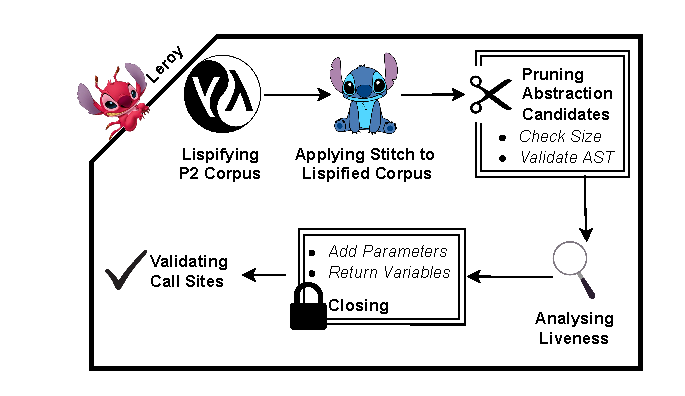
\includegraphics[width=\textwidth]{images/Design2.pdf}
  \caption{Architecture of the \toolname{} tool}
  \label{fig:design}
\end{figure*}


\subsection{Lispifying}
\label{sec:lispify}
To use Stitch, \toolname must first convert the \ptwo{} program into a Lisp-like representation understandable to Stitch. 
This conversion treats AST nodes as nested function calls, where each node acts as a function and its child nodes as arguments. This approach enables \toolname to unfold the AST into a single, unified function call, simplifying the abstraction process.
For instance, consider a Python AST representing the addition operation \code{1+2}. 
The AST would look like a tree (see Figure~\ref{figure:LibAbsAST}, with an 'add' node at the root and the constants `1' and `2' as its children. 
In a functional style, we can represent the tree as a function call $add(1, 2)$, where the left and right children are the first the second operands respectively. 
In a lisp-like form, this AST would appear as `(add 1 2)'. 

The other complication of lispifying is handling the imperative statements
of Python.  As an example, consider the following three statements \code{x=1;y=1;print(x+1)}. 
\toolname lispifies this sequence as $StatementList(x=1, StatementList(y=1, StatementList(print(x+y), \epsilon)))$, where $\epsilon$ is the empty statement. This encoding draws inspiration from the `let` statement in lisp. 



\subsection{Pruning Stitch's Abstractions}
Given the lispified code, Stitch suggests many candidate extracted functions that may not port well back to Python. To refine these candidates, \toolname prunes invalid candidates across a few categories. 

\subsubsection{Macro-Like Abstractions}
Stitch treats abstracted libraries effectively like macros, as it knows no better than to treat all program elements as first-class citizens. When a functionality is abstracted, it can simply be swapped with a call. This approach impacts program correctness as it results in incomplete abstractions, like abstracting ``\code{exp +}'' from ``\code{exp+exp}''. A potential abstraction ``\code{add(exp)}'' would replace an addition of ``\code{1+2}'' with the expression ``\code{add(1) 2}''. In Python, this is clearly invalid syntax. 

To identify and prune macro-like invalid candidates, \toolname attempts to reconstruct the candidate into a program AST form, then checks for the correctness of the yielded AST. ASTs are regenerated by inverting the lispify step from Section~\ref{sec:lispify}, that is, the $StatementList$ nodes are converted back into lists, and special keyword nodes are replaced with their corresponding Python AST nodes (e.g.\ an $Add$ operator).  

Once the reconstructed AST is built, we verify the completeness of the AST by ensuring all required child nodes of a parent node exist. Incomplete ASTs are indicative of macro-like structures leading them to be subsequently pruned. For example, an incomplete AST might involve a function call without required arguments, such as \code{add(a, )} where the second argument \code{b} is missing. 

\subsubsection{Invalid Parameters}
The search method of Stitch treats all tree nodes as potential ``holes'', that is, possible function parameters, which is incorrect in the case of Python whose AST nodes are not all first-class citizens. For example, when stitch abstracts over comparative sub-trees, like \code{x==y} or \code{x!=z} it can suggest abstractions that takes three parameters, two operands and a comparison operator. A potential candidate $f(x,op,y)$ would need to be called like: $f(x, ==, y)$ or $f(x, !=, y)$. As with macro-like abstractions, this candidate has invalid Python syntax.

To identify these cases, \toolname again analyzes the candidates’s body by converting it back into a Python AST and encoding parameters as identifier nodes. By validating these nodes against the AST structure, \toolname ensures the legitimacy of parameter usage within the candidate. For instance, in a comparison expression \code{(a > b)}, Stitch may produce an candidate of the form $compare(a, comparator, b)$ instead of $greater\_than(a,b)$.  Candidates that take invalid parameters are pruned out. 

\subsubsection{Presenting Non-trivial Abstractions}
Because Stitch optimizes on the abstracted function size relative to its use, it may abstract highly repeated single-line functionalities. Such functionality is found in abundance within the code-base, and unfortunately results in functions that, for example, simply adds two numbers.

To enhance the utility of suggested abstractions, \toolname filters out trivial cases by imposing a minimum size requirement. This criterion ensures that the extracted abstractions are sufficiently complex and meaningful to warrant inclusion. This enforces trivial functions, like simple addition or printing, are not abstracted alone despite having a high utility due to its high usage frequency. 

\label{closing}
\subsection{Closing Functions}

\subsubsection{Determining the Return Value}

Because Stitch treats abstractions as macros, it does not consider variable scoping in abstractions, which impacts code correctness in a language like Python. For example, Stitch can abstract assignments without returning the assignment targets. That is, it can suggest functions that change the value of a variable, but never returns the changed variable. In Python, such assignment will create a new variable local to the abstracted (called) function instead of changing the value of the variable from the calling function. This, although syntactically correct, changes the program behaviour.

\toolname complements the abstractions generated by Stitch by ensuring a useful return value. To find what needs to be returned, \toolname performs a liveness analysis across each candidate call site, to determine what variables are live out of the abstraction body. 
It is worth noting that the abstraction's parameters may themselves be live-out and need to be returned. If there are no variables live-out, \toolname reverts back to returning the last variable or expression in the abstraction’s body. Such an approach helps with functional correctness of the abstractions in the target programming language which may be used as sub-expressions at the call site. 
% For example, Stitch may produce an abstraction where a variable is updated, but does not return the variable at the end of the abstraction, thereby generating erroneous compressed code. 

\subsubsection{Determining Additional Parameters} 
Stitch's abstractions may assume the presence of certain variables, even if they are not passed into the abstraction, due to the disconnect between Python's imperative style and the lisp-like Stitch input language. 
% This is because the same variable names appear in similar code-fragments across different parts of of the corpus. 
It is important to pass these values as parameters to avoid uninitialized variables in the function body. To find these variables, \toolname uses the liveness analysis to determine variables that are not live into the abstraction's body. It is assumed that these variables exist in the calling scope, and they are added as parameters to the candidate.


\subsection{Validating Call Sites} %correctness
A final complication arising from Python's imperative nature is a possible renaming issue that emerges between a given call-site's arguments and the function body.
% Some abstraction calls may be invalid, as parameters passed to the abstraction may need to be recomputed within the abstraction's body. 
% Although we are able to find macro-like abstractions which are not valid Python ASTs, these abstraction calls can still be macro-like.
This problem is best illustrated with an example. Consider the candidate \code{print5(arg)} in Figure~\ref{fig:possible-invalid-function-call} on line~\ref{cd:candidate}. This function prints the value $arg$ five times. Stitch identifies that this abstraction could used instead of the loop on line~\ref{cd:callsite} by simply using the function call $print5(x)$ (line~\ref{cd:use}) --- but an application of the function here would be erroneous. 
However, this is an invalid call as $x$ is re-computed every iteration in the loop; but passing the value as $arg$ computes it only once at the call site. 

The issue here is an implicit renaming of the symbol ``x'' when aliased into an argument, that is, the value of ``x'' is used as the renamed ``arg'' (at line~\ref{cd:print}), but the name ``x'' has been lost otherwise (at line~\ref{cd:for}) and is no longer connected to the associated value.  Again, this issue arises from Python scoping rules diverging from lisp style programs.
To detect such invalid call-sites, \toolname analyzes each call site and its arguments, then validates that no names in the call site's arguments are referenced in the function, thereby preventing this name clash issue.

\begin{figure}
    \begin{lstlisting}
    def print5(arg):  # Verified Stitch candidate *@\label{cd:candidate}@*
        for x in range(5): *@\label{cd:for}@*
            print(arg) *@\label{cd:print}@*

    for x in range(5):   # Stitch identified usage (invalid) *@\label{cd:callsite}@*
        print(x)
        
    print5(x)   # Invalid candidate use (parameter and body overlap) *@\label{cd:use}@*
    \end{lstlisting}
    \caption{A valid function, which could be called erroneously}
    \label{fig:possible-invalid-function-call}
\end{figure}


% \subsection{Converting Abstractions back to the Programming Language AST}

% Finally, \toolname converts the refined suggestions from Stitch back into the Abstract Syntax Tree of the programming language. It then unparses the AST to yield the compressed code, integrating the identified abstractions seamlessly into the original program structure.
